\begin{figure}[t]
    \centering
    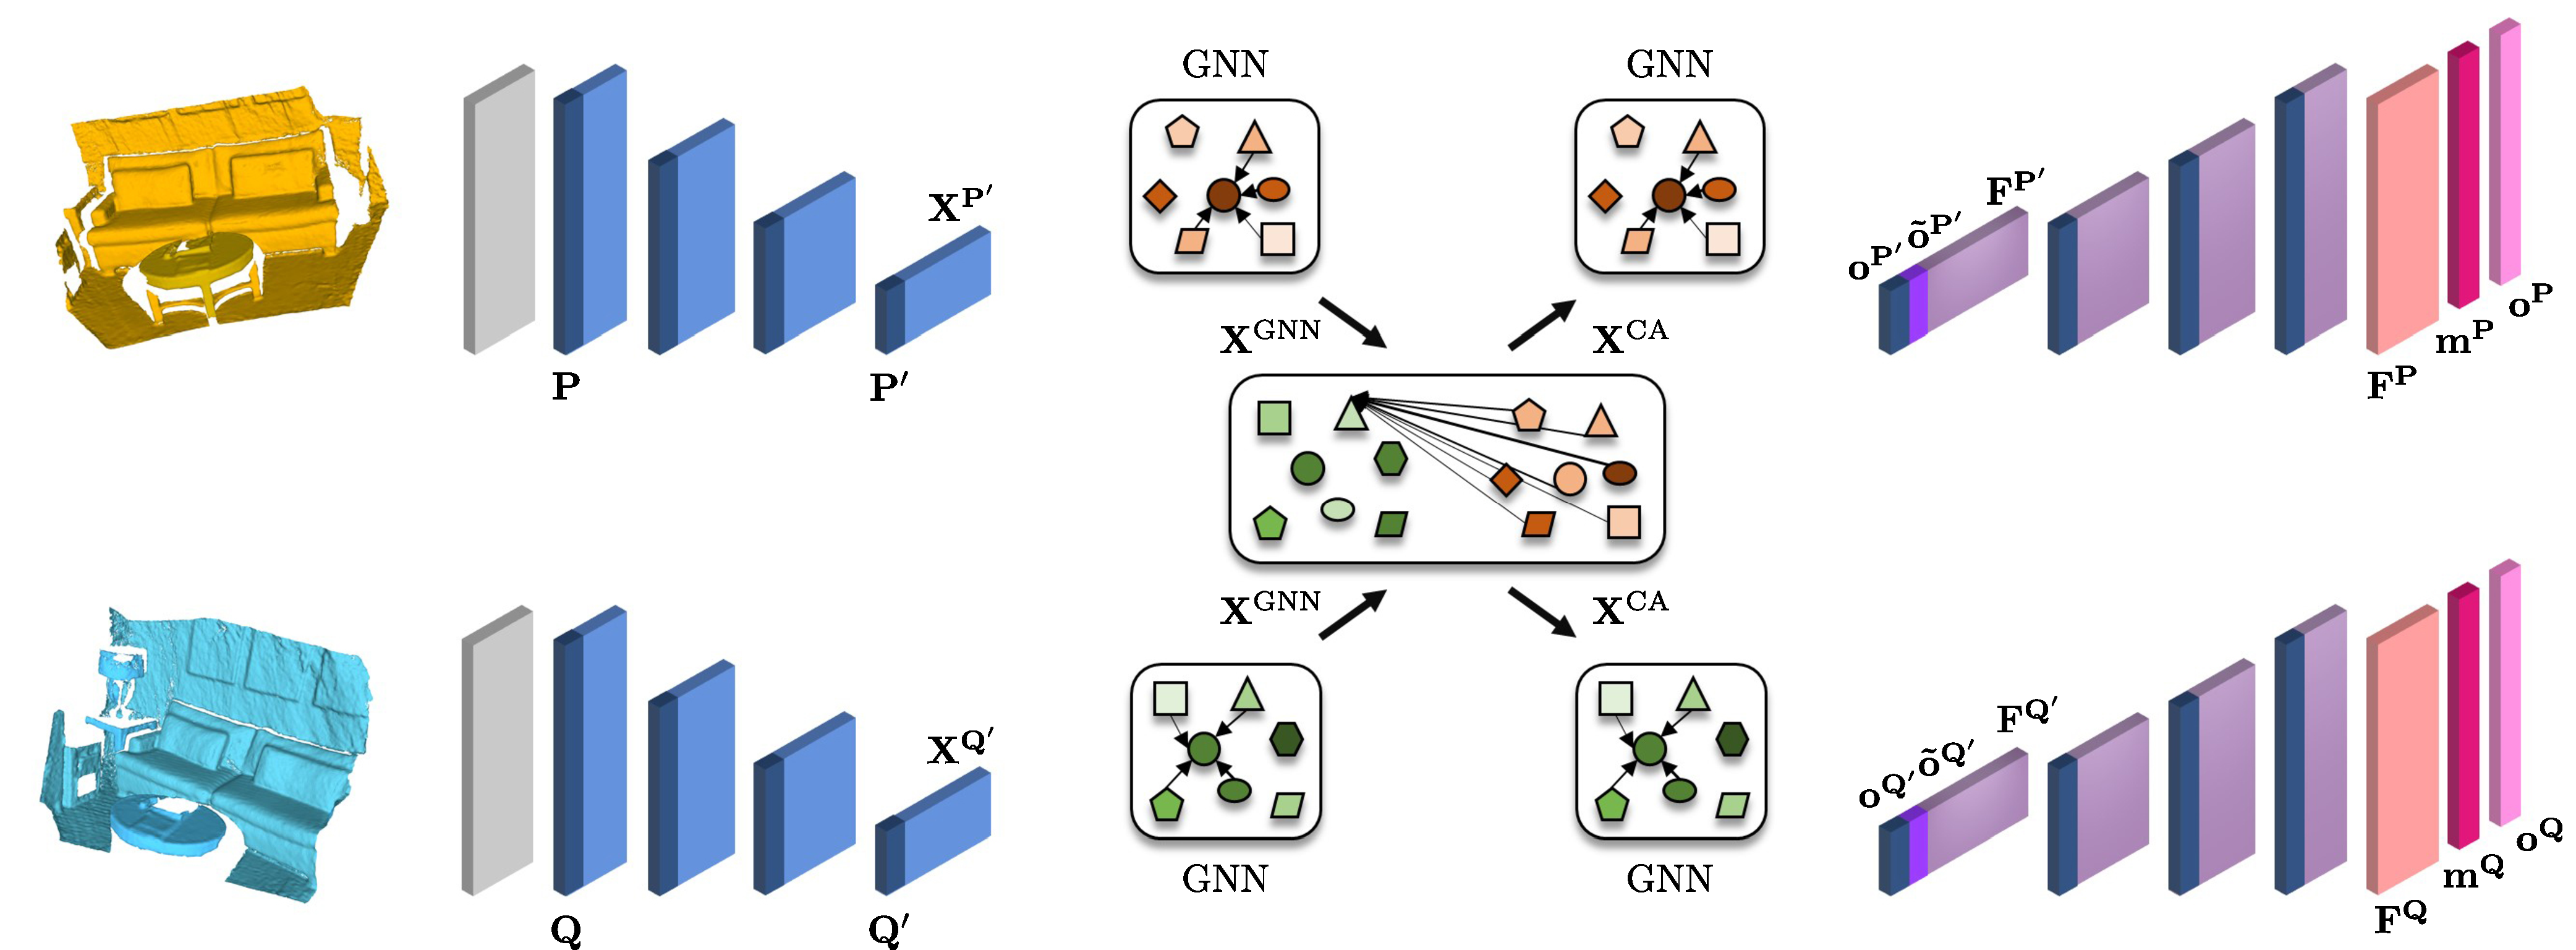
\includegraphics[width=1.0\columnwidth]{figures/images/network_architecture.pdf}
    \caption{Network architecture of \acro. \textcolor{gray}{Voxel-gridded} point clouds $\mathbf{P}$ and $\mathbf{Q}$ are fed to the encoder, which extracts the superpoints $\mathbf{P}'$ and $\mathbf{Q}'$ and their latent features $\mathbf{X}^{\mathbf{P}'}$, $\mathbf{X}^{\mathbf{Q}'}$. The overlap-attention module updates the features with co-contextual information in a series of self- (GNN) and cross-attention (CA) blocks, and projects them to overlap  $\mathbf{o}^{\mathbf{P}'}$, $\mathbf{o}^{\mathbf{Q}'}$ and cross-overlap $\tilde{\mathbf{o}}^{\mathbf{P}'}$, $\tilde{\mathbf{o}}^{\mathbf{Q}'}$ scores. Finally, the decoder transforms the conditioned features and overlap scores to per-point feature descriptors $\mathbf{F}^\mathbf{P}$, $\mathbf{F}^\mathbf{Q}$, overlap scores $\mathbf{o}^\mathbf{P}$, $\mathbf{o}^\mathbf{Q}$, and matchability scores $\mathbf{m}^\mathbf{P}$, $\mathbf{m}^\mathbf{Q}$.}
    \label{fig:network_arch}
    
\end{figure}